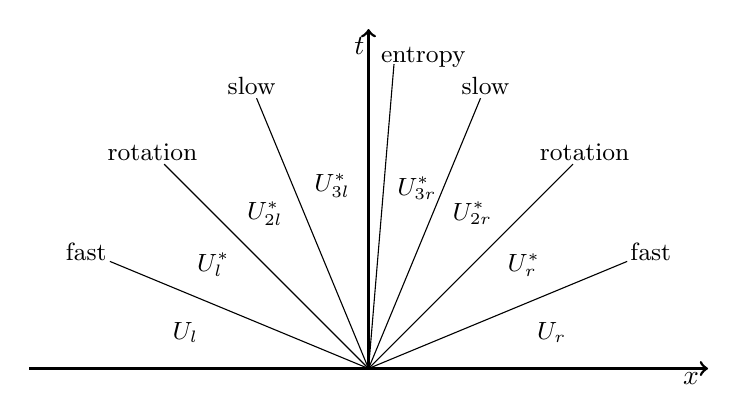
\begin{tikzpicture}[scale = {0.0125\linewidth},inner sep = 1pt]
%% \begin{tikzpicture}[scale = {0.015\linewidth},inner sep = 1pt]
%% \tikzstyle{every node} = [draw,circle,fill=gray!30];
%% \draw (-1.5,0.0) circle (0.8);
%% \draw[<->,line width=1pt] (0,1) node[right]{\;$t$}|-(1,0) node[below]{$m$};
\draw[line width=1pt] (0,0.95) node[left]{$t$}|-(0.95,0) node[below]{$x$};
\draw[->,line width=1pt] (0.95,0)--(1,0);
\draw[->,line width=1pt] (0,0.95)--(0,1);  
\draw[line width=1pt] (-0,0)--(-1,0);
\node[draw=white] (fr) at (0.83149,0.34442) {\small fast};
\node[draw=white] (rr) at (0.63640,0.63640) {\small rotation};
\node[draw=white] (sr) at (0.34442,0.83149) {\small slow};
%% \node[draw=white] (cd) at (0.17221,0.88337) {\small contact disc.};
\node[draw=white] (cd) at (0.16149,0.91587) {\small entropy};
\node[draw=white] (sl) at (-0.34442,0.83149) {\small slow};
\node[draw=white] (rl) at (-0.63640,0.63640) {\small rotation};
\node[draw=white] (fl) at (-0.83149,0.34442) {\small fast};

\node[draw=white] (R8a) at (0.53943,0.10730) {\small $\mbf{U}_{r}$};
\node[draw=white] (R7a) at (0.45731,0.30556) {\small $\mbf{U}^*_{r}$};
\node[draw=white] (R6a) at (0.30556,0.45731) {\small $\mbf{U}^*_{2r}$};
\node[draw=white] (R5a) at (0.14235,0.53126) {\small $\mbf{U}^*_{3r}$};
\node[draw=white] (R4a) at (-0.10730,0.53943) {\small $\mbf{U}^*_{3l}$};
\node[draw=white] (R3a) at (-0.30556,0.45731) {\small $\mbf{U}^*_{2l}$};
\node[draw=white] (R2a) at (-0.45731,0.30556) {\small $\mbf{U}^*_{l}$};
\node[draw=white] (R1a) at (-0.53943,0.10730) {\small $\mbf{U}_{l}$};

%% \node[] at (0.15,0.95) {contact};
\draw (0,0) -- (fr);  
\draw (0,0) -- (rr);  
\draw (0,0) -- (sr);  
\draw (0,0) -- (0.075,0.89678);  
\draw (0,0) -- (sl);  
\draw (0,0) -- (rl);  
\draw (0,0) -- (fl);  
\end{tikzpicture}
